\documentclass{article}

% if you need to pass options to natbib, use, e.g.:
%     \PassOptionsToPackage{numbers, compress}{natbib}
% before loading neurips_2024


% ready for submission
\usepackage[final]{neurips_2024}


% to compile a preprint version, e.g., for submission to arXiv, add add the
% [preprint] option:
%     \usepackage[preprint]{neurips_2024}


% to compile a camera-ready version, add the [final] option, e.g.:
%     \usepackage[final]{neurips_2024}


% to avoid loading the natbib package, add option nonatbib:
%    \usepackage[nonatbib]{neurips_2024}


\usepackage[utf8]{inputenc} % allow utf-8 input
\usepackage[T1]{fontenc}    % use 8-bit T1 fonts
\usepackage{hyperref}       % hyperlinks
\usepackage{url}            % simple URL typesetting
\usepackage{booktabs}       % professional-quality tables
\usepackage{amsfonts}       % blackboard math symbols
\usepackage{nicefrac}       % compact symbols for 1/2, etc.
\usepackage{microtype}      % microtypography
\usepackage{xcolor}         % colors
\usepackage{pgfplots}
\usepackage{pgfplotstable} % If using table data
\pgfplotsset{compat=1.18}


\title{\LaTeX\ Template for GSHS Final Report}


% The \author macro works with any number of authors. There are two commands
% used to separate the names and addresses of multiple authors: \And and \AND.
%
% Using \And between authors leaves it to LaTeX to determine where to break the
% lines. Using \AND forces a line break at that point. So, if LaTeX puts 3 of 4
% authors names on the first line, and the last on the second line, try using
% \AND instead of \And before the third author name.


\author{%
  Firstname Lastname \\
  Institution \\
  \texttt{username@domain.edu} \\
  % examples of more authors
  % \And
  % Coauthor \\
  % Affiliation \\
  % Address \\
  % \texttt{email} \\
  % \AND
  % Coauthor \\
  % Affiliation \\
  % Address \\
  % \texttt{email} \\
  % \And
  % Coauthor \\
  % Affiliation \\
  % Address \\
  % \texttt{email} \\
  % \And
  % Coauthor \\
  % Affiliation \\
  % Address \\
  % \texttt{email} \\
}


\begin{document}


\maketitle

(remove this paragraph when submitting)
\begin{enumerate}
\item Due: By the end of January 18, 2026.
\item Update name, institution, and email address above.
\item Fill out all sections according to the instructions below.
\item Generate a plot using a provided template.
\item Page limit: 2 pages. You must not exceed 2 pages excluding references. 
    At the same time, it should be longer than about 1.5 pages at least. 
\item Feel free to import any additional libraries
\end{enumerate}


\section{Introduction (0.5 pages)}

The introduction should provide background and motivation for studying the scalability of Gradient Descent in real-world machine learning systems. This section should be
organized as follows:

(1) Briefly talk about how Gradient Descent serves as an important optimization algorithm for training machine learning models.

(2) State the main goal of this project: to experimentally investigate the scalability of Gradient Descent as the problem size increases.

To cite any websites like \citep{gd_wiki},
    add bibtex entries to the file named \texttt{references.bib}
        and use either \texttt{\textbackslash cite} or \texttt{\textbackslash citep} command.


\section{Experimental Setup (0.5 pages)}

Describe the methodologies of the different experiments performed to evaluate scalability, and explain how each experiment is designed to isolate and measure a specific scalability factor.

You may describe the underlying optimization problem (linear regression with Mean Squared Error), the datasets used, and the range of dataset sizes and feature dimensions considered.


\clearpage

\section{Results (0.8 pages)}

\begin{figure}[t]
\centering

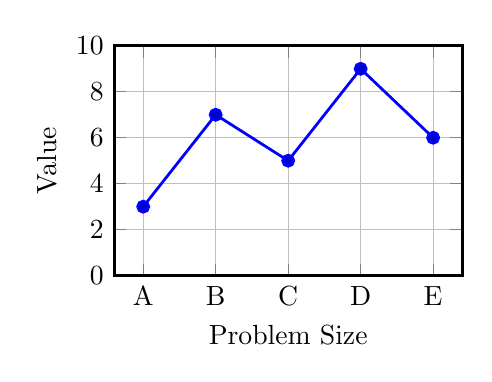
\begin{tikzpicture}
    \begin{axis}[
        width=60mm,
        height=45mm,
        xlabel={Problem Size},
        ylabel={Value},
        ymin=0,
        ymax=10,
        symbolic x coords={A, B, C, D, E},
        xtick=data,
        grid=major,
        mark=*,
        line width=1pt
    ]
        \addplot coordinates {(A,3) (B,7) (C,5) (D,9) (E,6)};
    \end{axis}
\end{tikzpicture}

\caption{Describe your figure using a few sentences.}
\end{figure}


Present and discuss your experimental results using the provided plotting template. Additional figures may be included if necessary (Consider using the subfigure environment to arrange multiple plots in a single row).


\section{Conclusion (0.2 pages)}

Summarize the main findings of the scalability study and discuss the limitations of full batch gradient descent.

\clearpage

\bibliographystyle{plainnat} % Standard NeurIPS style
\bibliography{references} % Link to your .bib file

\end{document}
